% Options for packages loaded elsewhere
\PassOptionsToPackage{unicode}{hyperref}
\PassOptionsToPackage{hyphens}{url}
%
\documentclass[
  ignorenonframetext,
]{beamer}
\usepackage{pgfpages}
\setbeamertemplate{caption}[numbered]
\setbeamertemplate{caption label separator}{: }
\setbeamercolor{caption name}{fg=normal text.fg}
\beamertemplatenavigationsymbolsempty
% Prevent slide breaks in the middle of a paragraph
\widowpenalties 1 10000
\raggedbottom
\setbeamertemplate{part page}{
  \centering
  \begin{beamercolorbox}[sep=16pt,center]{part title}
    \usebeamerfont{part title}\insertpart\par
  \end{beamercolorbox}
}
\setbeamertemplate{section page}{
  \centering
  \begin{beamercolorbox}[sep=12pt,center]{part title}
    \usebeamerfont{section title}\insertsection\par
  \end{beamercolorbox}
}
\setbeamertemplate{subsection page}{
  \centering
  \begin{beamercolorbox}[sep=8pt,center]{part title}
    \usebeamerfont{subsection title}\insertsubsection\par
  \end{beamercolorbox}
}
\AtBeginPart{
  \frame{\partpage}
}
\AtBeginSection{
  \ifbibliography
  \else
    \frame{\sectionpage}
  \fi
}
\AtBeginSubsection{
  \frame{\subsectionpage}
}

\usepackage{amsmath,amssymb}
\usepackage{iftex}
\ifPDFTeX
  \usepackage[T1]{fontenc}
  \usepackage[utf8]{inputenc}
  \usepackage{textcomp} % provide euro and other symbols
\else % if luatex or xetex
  \usepackage{unicode-math}
  \defaultfontfeatures{Scale=MatchLowercase}
  \defaultfontfeatures[\rmfamily]{Ligatures=TeX,Scale=1}
\fi
\usepackage{lmodern}
\usecolortheme{Flip}
\usefonttheme{serif} % use mainfont rather than sansfont for slide text
\useinnertheme{Flip}
\useoutertheme{Flip}
\ifPDFTeX\else  
    % xetex/luatex font selection
  \setmainfont[]{VisbyCF-Medium}
  \setsansfont[]{Latin Modern Sans}
  \setmathfont[]{Latin Modern Math}
\fi
% Use upquote if available, for straight quotes in verbatim environments
\IfFileExists{upquote.sty}{\usepackage{upquote}}{}
\IfFileExists{microtype.sty}{% use microtype if available
  \usepackage[]{microtype}
  \UseMicrotypeSet[protrusion]{basicmath} % disable protrusion for tt fonts
}{}
\makeatletter
\@ifundefined{KOMAClassName}{% if non-KOMA class
  \IfFileExists{parskip.sty}{%
    \usepackage{parskip}
  }{% else
    \setlength{\parindent}{0pt}
    \setlength{\parskip}{6pt plus 2pt minus 1pt}}
}{% if KOMA class
  \KOMAoptions{parskip=half}}
\makeatother
\usepackage{xcolor}
\newif\ifbibliography
\setlength{\emergencystretch}{3em} % prevent overfull lines
\setcounter{secnumdepth}{-\maxdimen} % remove section numbering

\usepackage{color}
\usepackage{fancyvrb}
\newcommand{\VerbBar}{|}
\newcommand{\VERB}{\Verb[commandchars=\\\{\}]}
\DefineVerbatimEnvironment{Highlighting}{Verbatim}{commandchars=\\\{\}}
% Add ',fontsize=\small' for more characters per line
\usepackage{framed}
\definecolor{shadecolor}{RGB}{241,243,245}
\newenvironment{Shaded}{\begin{snugshade}}{\end{snugshade}}
\newcommand{\AlertTok}[1]{\textcolor[rgb]{0.68,0.00,0.00}{#1}}
\newcommand{\AnnotationTok}[1]{\textcolor[rgb]{0.37,0.37,0.37}{#1}}
\newcommand{\AttributeTok}[1]{\textcolor[rgb]{0.40,0.45,0.13}{#1}}
\newcommand{\BaseNTok}[1]{\textcolor[rgb]{0.68,0.00,0.00}{#1}}
\newcommand{\BuiltInTok}[1]{\textcolor[rgb]{0.00,0.23,0.31}{#1}}
\newcommand{\CharTok}[1]{\textcolor[rgb]{0.13,0.47,0.30}{#1}}
\newcommand{\CommentTok}[1]{\textcolor[rgb]{0.37,0.37,0.37}{#1}}
\newcommand{\CommentVarTok}[1]{\textcolor[rgb]{0.37,0.37,0.37}{\textit{#1}}}
\newcommand{\ConstantTok}[1]{\textcolor[rgb]{0.56,0.35,0.01}{#1}}
\newcommand{\ControlFlowTok}[1]{\textcolor[rgb]{0.00,0.23,0.31}{#1}}
\newcommand{\DataTypeTok}[1]{\textcolor[rgb]{0.68,0.00,0.00}{#1}}
\newcommand{\DecValTok}[1]{\textcolor[rgb]{0.68,0.00,0.00}{#1}}
\newcommand{\DocumentationTok}[1]{\textcolor[rgb]{0.37,0.37,0.37}{\textit{#1}}}
\newcommand{\ErrorTok}[1]{\textcolor[rgb]{0.68,0.00,0.00}{#1}}
\newcommand{\ExtensionTok}[1]{\textcolor[rgb]{0.00,0.23,0.31}{#1}}
\newcommand{\FloatTok}[1]{\textcolor[rgb]{0.68,0.00,0.00}{#1}}
\newcommand{\FunctionTok}[1]{\textcolor[rgb]{0.28,0.35,0.67}{#1}}
\newcommand{\ImportTok}[1]{\textcolor[rgb]{0.00,0.46,0.62}{#1}}
\newcommand{\InformationTok}[1]{\textcolor[rgb]{0.37,0.37,0.37}{#1}}
\newcommand{\KeywordTok}[1]{\textcolor[rgb]{0.00,0.23,0.31}{#1}}
\newcommand{\NormalTok}[1]{\textcolor[rgb]{0.00,0.23,0.31}{#1}}
\newcommand{\OperatorTok}[1]{\textcolor[rgb]{0.37,0.37,0.37}{#1}}
\newcommand{\OtherTok}[1]{\textcolor[rgb]{0.00,0.23,0.31}{#1}}
\newcommand{\PreprocessorTok}[1]{\textcolor[rgb]{0.68,0.00,0.00}{#1}}
\newcommand{\RegionMarkerTok}[1]{\textcolor[rgb]{0.00,0.23,0.31}{#1}}
\newcommand{\SpecialCharTok}[1]{\textcolor[rgb]{0.37,0.37,0.37}{#1}}
\newcommand{\SpecialStringTok}[1]{\textcolor[rgb]{0.13,0.47,0.30}{#1}}
\newcommand{\StringTok}[1]{\textcolor[rgb]{0.13,0.47,0.30}{#1}}
\newcommand{\VariableTok}[1]{\textcolor[rgb]{0.07,0.07,0.07}{#1}}
\newcommand{\VerbatimStringTok}[1]{\textcolor[rgb]{0.13,0.47,0.30}{#1}}
\newcommand{\WarningTok}[1]{\textcolor[rgb]{0.37,0.37,0.37}{\textit{#1}}}

\providecommand{\tightlist}{%
  \setlength{\itemsep}{0pt}\setlength{\parskip}{0pt}}\usepackage{longtable,booktabs,array}
\usepackage{calc} % for calculating minipage widths
\usepackage{caption}
% Make caption package work with longtable
\makeatletter
\def\fnum@table{\tablename~\thetable}
\makeatother
\usepackage{graphicx}
\makeatletter
\def\maxwidth{\ifdim\Gin@nat@width>\linewidth\linewidth\else\Gin@nat@width\fi}
\def\maxheight{\ifdim\Gin@nat@height>\textheight\textheight\else\Gin@nat@height\fi}
\makeatother
% Scale images if necessary, so that they will not overflow the page
% margins by default, and it is still possible to overwrite the defaults
% using explicit options in \includegraphics[width, height, ...]{}
\setkeys{Gin}{width=\maxwidth,height=\maxheight,keepaspectratio}
% Set default figure placement to htbp
\makeatletter
\def\fps@figure{htbp}
\makeatother

\usepackage{booktabs}
\usepackage{caption}
\usepackage{longtable}
\usepackage{tabu}
\usepackage{mathtools}
\usepackage{mathrsfs}
\makeatletter
\makeatother
\makeatletter
\makeatother
\makeatletter
\@ifpackageloaded{caption}{}{\usepackage{caption}}
\AtBeginDocument{%
\ifdefined\contentsname
  \renewcommand*\contentsname{Table of contents}
\else
  \newcommand\contentsname{Table of contents}
\fi
\ifdefined\listfigurename
  \renewcommand*\listfigurename{List of Figures}
\else
  \newcommand\listfigurename{List of Figures}
\fi
\ifdefined\listtablename
  \renewcommand*\listtablename{List of Tables}
\else
  \newcommand\listtablename{List of Tables}
\fi
\ifdefined\figurename
  \renewcommand*\figurename{Figure}
\else
  \newcommand\figurename{Figure}
\fi
\ifdefined\tablename
  \renewcommand*\tablename{Table}
\else
  \newcommand\tablename{Table}
\fi
}
\@ifpackageloaded{float}{}{\usepackage{float}}
\floatstyle{ruled}
\@ifundefined{c@chapter}{\newfloat{codelisting}{h}{lop}}{\newfloat{codelisting}{h}{lop}[chapter]}
\floatname{codelisting}{Listing}
\newcommand*\listoflistings{\listof{codelisting}{List of Listings}}
\makeatother
\makeatletter
\@ifpackageloaded{caption}{}{\usepackage{caption}}
\@ifpackageloaded{subcaption}{}{\usepackage{subcaption}}
\makeatother
\makeatletter
\@ifpackageloaded{tcolorbox}{}{\usepackage[skins,breakable]{tcolorbox}}
\makeatother
\makeatletter
\@ifundefined{shadecolor}{\definecolor{shadecolor}{rgb}{.97, .97, .97}}
\makeatother
\makeatletter
\makeatother
\makeatletter
\makeatother
\ifLuaTeX
  \usepackage{selnolig}  % disable illegal ligatures
\fi
\IfFileExists{bookmark.sty}{\usepackage{bookmark}}{\usepackage{hyperref}}
\IfFileExists{xurl.sty}{\usepackage{xurl}}{} % add URL line breaks if available
\urlstyle{same} % disable monospaced font for URLs
\hypersetup{
  pdftitle={Régression logistique},
  pdfauthor={Léo Belzile},
  hidelinks,
  pdfcreator={LaTeX via pandoc}}

\title{Régression logistique}
\subtitle{Analyse multidimensionnelle appliquée}
\author{Léo Belzile}
\date{}
\institute{HEC Montréal}

\begin{document}
\frame{\titlepage}
\ifdefined\Shaded\renewenvironment{Shaded}{\begin{tcolorbox}[frame hidden, borderline west={3pt}{0pt}{shadecolor}, enhanced, boxrule=0pt, breakable, sharp corners, interior hidden]}{\end{tcolorbox}}\fi

\begin{frame}{\emph{Professional Rodeo Cowboys Association}}
\protect\hypertarget{cowboy}{}
L'exemple suivant est inspiré de l'article

\begin{quote}
Daneshvary, R. et Schwer, R. K. (2000) The Association Endorsement and
Consumers' Intention to Purchase. \emph{Journal of Consumer Marketing}
\textbf{17}, 203-213.
\end{quote}

\textbf{Objectif}: Les auteurs cherchent à voir si le fait qu'un produit
soit recommandé par le \emph{Professional Rodeo Cowboys Association}
(PRCA) a un effet sur les intentions d'achats.
\end{frame}

\begin{frame}[fragile]{Données du PRCA}
\protect\hypertarget{donnuxe9es-du-prca}{}
On dispose de 500 observations sur les variables suivantes dans la base
de données \texttt{logit1}: \footnotesize 

\begin{itemize}
\tightlist
\item
  \(Y\): seriez-vous intéressé à acheter un produit recommandé par le
  PRCA

  \begin{itemize}
  \tightlist
  \item
    \(\texttt{0}\): non
  \item
    \(\texttt{1}\): oui
  \end{itemize}
\item
  \(\mathrm{X}_1\): quel genre d'emploi occupez-vous?

  \begin{itemize}
  \tightlist
  \item
    \(\texttt{1}\): à la maison
  \item
    \(\texttt{2}\): employé
  \item
    \(\texttt{3}\): ventes/services
  \item
    \(\texttt{4}\): professionnel
  \item
    \(\texttt{5}\): agriculture/ferme
  \end{itemize}
\item
  \(\mathrm{X}_2\): revenu familial annuel

  \begin{itemize}
  \tightlist
  \item
    \(\texttt{1}\): moins de 25 000
  \item
    \(\texttt{2}\): 25 000 à 39 999
  \item
    \(\texttt{3}\): 40 000 à 59 999
  \item
    \(\texttt{4}\): 60 000 à 79 999
  \item
    \(\texttt{5}\): 80 000 et plus
  \end{itemize}
\end{itemize}

\normalsize
\end{frame}

\begin{frame}{Données du PRCA}
\protect\hypertarget{donnuxe9es-du-prca-1}{}
\footnotesize

\begin{itemize}
\tightlist
\item
  \(\mathrm{X}_3\): sexe

  \begin{itemize}
  \tightlist
  \item
    \(\texttt{0}\): homme
  \item
    \(\texttt{1}\): femme
  \end{itemize}
\item
  \(\mathrm{X}_4\): avez-vous déjà fréquenté une université?

  \begin{itemize}
  \tightlist
  \item
    \(\texttt{0}\): non
  \item
    \(\texttt{1}\): oui
  \end{itemize}
\item
  \(\mathrm{X}_5\): âge (en années)
\item
  \(\mathrm{X}_6\): combien de fois avez-vous assisté à un rodéo au
  cours de la dernière année?

  \begin{itemize}
  \tightlist
  \item
    \(\texttt{1}\): 10 fois ou plus
  \item
    \(\texttt{2}\): entre six et neuf fois
  \item
    \(\texttt{3}\): cinq fois ou moins
  \end{itemize}
\end{itemize}

\normalsize
\end{frame}

\begin{frame}{Régression logistique}
\protect\hypertarget{ruxe9gression-logistique}{}
Expliquer le comportement de la \textbf{moyenne} d'une variable binaire
\(Y\in\{0,1\}\) en utilisant un modèle de régression avec \(p\)
variables explicatives \(\mathrm{X}_1, \ldots, \mathrm{X}_p\).

\[\underset{\text{moyenne théorique}}{\mathsf{E}(Y=1 \mid \mathbf{X})} = \underset{\text{probabilité de succès}}{\Pr(Y=1 \mid \mathbf{X})}=p\]
\end{frame}

\begin{frame}{Objectif de la régression}
\protect\hypertarget{objectif-de-la-ruxe9gression}{}
\begin{enumerate}
[1)]
\tightlist
\item
  \textbf{Inférence} : comprendre comment et dans quelles mesures les
  variables \(\mathbf{X}\) influencent la probabilité que \(Y=1\).
\item
  \textbf{Prédiction} : développer un modèle pour prévoir des valeurs de
  \(Y\) ou la probabilité de succès à partir des \(\mathbf{X}\).
\end{enumerate}
\end{frame}

\begin{frame}{Exemples}
\protect\hypertarget{exemples}{}
\begin{itemize}
\tightlist
\item
  Est-ce qu'un client potentiel va répondre favorablement à une offre
  promotionnelle?
\item
  Est-ce qu'un client est satisfait du service après-vente?
\item
  Est-ce qu'un client va faire faillite ou non au cours des trois
  prochaines années.
\end{itemize}
\end{frame}

\begin{frame}{Inférence et interprétation}
\protect\hypertarget{infuxe9rence-et-interpruxe9tation}{}
Ce cours est consacré à l'estimation et l'interprétation des paramètres
du modèle dans le cas binaire.

Par convention, on désigne le résultat « \(1\) » par un succès et «
\(0\) » par un échec.
\end{frame}

\begin{frame}{Modéliser une probabilité avec une régression linéaire?}
\protect\hypertarget{moduxe9liser-une-probabilituxe9-avec-une-ruxe9gression-linuxe9aire}{}
Mauvaise idée!

\begin{itemize}
\tightlist
\item
  Sans contrainte, on peut obtenir des probabilités négatives ou
  supérieures à 1!
\item
  les données binaires ne respectent pas le postulat d'égalité des
  variances

  \begin{itemize}
  \tightlist
  \item
    invalide les résultats des tests d'hypothèse pour les coefficients.
  \end{itemize}
\end{itemize}
\end{frame}

\begin{frame}{Illustration: linéaire vs logistique}
\protect\hypertarget{illustration-linuxe9aire-vs-logistique}{}
\begin{figure}

{\centering \includegraphics[width=0.8\textwidth,height=\textheight]{MATH60602-diapos5_files/figure-beamer/fig-demandecredit-1.pdf}

}

\caption{\label{fig-demandecredit}Données de la réserve de Boston sur
l'approbation de prêts hypothécaires (1990); données tirées de Stock et
Watson (2007).}

\end{figure}
\end{frame}

\begin{frame}{Fonction de liaison}
\protect\hypertarget{fonction-de-liaison}{}
Idée: appliquer une transformation au \textbf{prédicteur linéaire}
\[\eta = \beta_0 + \beta_1 \mathrm{X}_1 + \cdots + \beta_p \mathrm{X}_p\]
pour que la prédiction soit entre zéro et un.

On considère \begin{align*}
 p &= \textrm{expit}(\eta) = \frac{\exp(\eta)}{1+\exp(\eta)}
= \frac{1}{1+\exp(-\eta)}.
\end{align*}
\end{frame}

\begin{frame}{Courbe sigmoïde}
\protect\hypertarget{courbe-sigmouxefde}{}
\begin{figure}

{\centering \includegraphics[width=0.9\textwidth,height=\textheight]{MATH60602-diapos5_files/figure-beamer/fig-logitplot-1.pdf}

}

\caption{\label{fig-logitplot}Valeurs ajustées du modèle de régression
logistique en fonction du prédicteur linéaire \(\eta\).}

\end{figure}
\end{frame}

\begin{frame}[fragile]{Ajustement du modèle}
\protect\hypertarget{ajustement-du-moduxe8le}{}
La fonction \texttt{glm} dans \textbf{R} ajuste un modèle linéaire
généralisé (par défaut, Gaussien pour régression linéaire).

\begin{itemize}
\tightlist
\item
  L'argument \texttt{family=binomial(link="logit")} permet de spécifier
  que l'on ajuste un modèle logistique.
\end{itemize}

\begin{Shaded}
\begin{Highlighting}[numbers=left,,]
\FunctionTok{data}\NormalTok{(logit1, }\AttributeTok{package =} \StringTok{"hecmulti"}\NormalTok{)}
\CommentTok{\# Ajustement du modèle avec toutes}
\CommentTok{\# les variables explicatives}
\NormalTok{modele1 }\OtherTok{\textless{}{-}} \FunctionTok{glm}\NormalTok{(}\AttributeTok{formula =}\NormalTok{ y }\SpecialCharTok{\textasciitilde{}}\NormalTok{ .,}
            \AttributeTok{family =} \FunctionTok{binomial}\NormalTok{(}\AttributeTok{link =} \StringTok{"logit"}\NormalTok{),}
            \AttributeTok{data =}\NormalTok{ logit1)}
\end{Highlighting}
\end{Shaded}
\end{frame}

\begin{frame}[fragile]{Sortie}
\protect\hypertarget{sortie}{}
Tableau résumé avec les coefficients (\texttt{summary})

\begin{Shaded}
\begin{Highlighting}[numbers=left,,]
\FunctionTok{summary}\NormalTok{(modele1)}
\end{Highlighting}
\end{Shaded}
\end{frame}

\begin{frame}{Interprétation}
\protect\hypertarget{interpruxe9tation}{}
Par défaut, pour des variables \(0/1\), le modèle décrit la probabilité
de succès.

\begin{figure}

{\centering \includegraphics[width=0.7\textwidth,height=\textheight]{MATH60602-diapos5_files/figure-beamer/logitplot2-1.pdf}

}

\end{figure}

Si le coefficient \(\beta_j\) de la variable \(\mathrm{X}_j\) est
positif, alors plus la variable augmente, plus \(\Pr(Y=1)\) augmente.
\end{frame}

\begin{frame}{Rappel exponentiels et logarithme}
\protect\hypertarget{rappel-exponentiels-et-logarithme}{}
Quelques propriétés de la fonction exponentielle:

\begin{itemize}
\tightlist
\item
  \(\exp(0) = 1\)
\item
  \(\exp(a + b) = \exp(a)\exp(b)\)
\item
  \(\exp(ab)= \exp(a)^b\)
\end{itemize}

Quelques propriétés de la fonction logarithmique

\begin{itemize}
\tightlist
\item
  \(\ln(1)=0\),
\item
  \(\ln(\exp(x))=x\) (fonction inverse)
\item
  \(\ln(ab) = \ln(a) + \ln(b)\)
\end{itemize}
\end{frame}

\begin{frame}{Cote}
\protect\hypertarget{cote}{}
Si on applique la transformation inverse, on obtient

\[\ln\left(\frac{p}{1-p} \right) = \eta = \beta_0 + \beta_1 \mathrm{X}_1 + \cdots + \beta_p \mathrm{X}_p.\]

ou, en prenant l'exponentielle de chaque côté,

\[ 
\mathsf{cote} = \frac{p}{1-p} = \exp(\beta_0)\cdots\exp(\beta_p \mathrm{X}_p)
\]

\textbf{Modèle multiplicatif} pour la cote.
\end{frame}

\begin{frame}{Cote et probabilité}
\protect\hypertarget{cote-et-probabilituxe9}{}
La cote est utilisée dans les paris sportifs \begin{align*}
 \mathsf{cote}(p) = \frac{p}{1-p} = \frac{\Pr(Y=1 \mid \mathbf{X})}{\Pr(Y=0 \mid \mathbf{X})}.
\end{align*}

\hypertarget{tbl-cotes}{}
\begin{table}
\caption{\label{tbl-cotes}Cote et probabilité de succès }\tabularnewline

\centering
\begin{tabular}{lccccccccc}
\toprule
\(p\) & 0.1 & 0.2 & 0.3 & 0.4 & 0.5 & 0.6 & 0.7 & 0.8 & 0.9\\
\midrule
cote & \(\frac{1}{9}\) & \(\frac{1}{4}\) & \(\frac{3}{7}\) & \(\frac{2}{3}\) & \(1\) & \(\frac{3}{2}\) & \(\frac{7}{3}\) & \(4\) & \(9\)\\
\bottomrule
\end{tabular}
\end{table}
\end{frame}

\begin{frame}{Interprétation avec données du PRCA}
\protect\hypertarget{interpruxe9tation-avec-donnuxe9es-du-prca}{}
Le modèle ajusté en termes de cote est \begin{align*}
 \frac{\Pr(Y=1 \mid \mathrm{X}_5=x_5)}{\Pr(Y=0 \mid \mathrm{X}_5=x_5)} = \exp(-3.05)\exp(0.0749x_5).
\end{align*}

\small

\begin{itemize}
\tightlist
\item
  Lorsque \(\mathrm{X}_5\) augmente d'une année, la cote est multipliée
  par \(\exp(0.0749) = 1.078\) peut importe la valeur de \(x_5\).
\item
  Pour deux personnes dont la différence d'âge

  \begin{itemize}
  \tightlist
  \item
    est d'un an, la cote de la personne plus âgée est 7.8\% plus élevée
  \item
    est de 10 ans, la cote de la personne plus âgée est 112\% plus
    élevée (cote multipliée par
    \(\exp(10 \times 0.0749)=1.078^{10} = 2.12\))
  \end{itemize}
\end{itemize}

\normalsize
\end{frame}

\begin{frame}[fragile]{Modèle complet}
\protect\hypertarget{moduxe8le-complet}{}
On considère le modèle avec toutes les variables explicatives:

\begin{Shaded}
\begin{Highlighting}[numbers=left,,]
\NormalTok{modele2 }\OtherTok{\textless{}{-}} \FunctionTok{glm}\NormalTok{(}
  \AttributeTok{formula =}\NormalTok{ y }\SpecialCharTok{\textasciitilde{}}\NormalTok{ .,}
  \AttributeTok{data =}\NormalTok{ logit1,}
  \AttributeTok{family =}\NormalTok{ binomial)}
\FunctionTok{exp}\NormalTok{(}\FunctionTok{coef}\NormalTok{(modele2))}
\end{Highlighting}
\end{Shaded}

\begin{verbatim}
(Intercept)         x12         x13         x14         x15         x22 
      0.062       0.438       0.512       0.509       0.699       0.833 
        x23         x24         x25          x3          x4          x5 
      0.572       0.087       0.264       3.854       6.236       1.116 
        x62         x63 
      0.255       0.090 
\end{verbatim}
\end{frame}

\begin{frame}{Interprétation des coefficients}
\protect\hypertarget{interpruxe9tation-des-coefficients}{}
Si on a plusieurs variables explicatives, les coefficients sont
interprétés en modifiant une variable à la fois.

On compare deux profils identiques, sauf pour la variable en question

\begin{itemize}
\tightlist
\item
  toute chose étant égale par ailleurs
\item
  \emph{ceteris paribus}
\end{itemize}
\end{frame}

\begin{frame}{Interprétation des coefficients}
\protect\hypertarget{interpruxe9tation-des-coefficients-1}{}
\textbf{Variable continue}:

\begin{itemize}
\tightlist
\item
  La cote de la personne plus âgée d'un an est 1.116 fois celle de la
  personne plus jeune, \emph{ceteris paribus}, une augmentation de
  11,6\%
\end{itemize}
\end{frame}

\begin{frame}[fragile]{Variable binaire}
\protect\hypertarget{variable-binaire}{}
Le rapport de cote pour les femmes (\texttt{x3=1}) versus les hommes
(\texttt{x3=0}) est de \(\exp(\widehat{\beta}_{\mathrm{X}_3}) = 3.854\):

\begin{itemize}
\tightlist
\item
  les femmes sont plus susceptibles de suivre les recommendations
  d'achat toute chose étant égale par ailleurs,
\item
  Inversement, le rapport de cote homme/femme est de 1/3.854=0.259,
\end{itemize}

On peut donc conclure que:

\begin{itemize}
\tightlist
\item
  la cote des femmes est 285.4\% plus élevée que celle des hommes.
\item
  la cote des hommes est 74.1\% inférieure à celle des femmes.
\end{itemize}
\end{frame}

\begin{frame}[fragile]{Variable catégorielle}
\protect\hypertarget{variable-catuxe9gorielle}{}
Toutes les comparaisons sont effectuées avec la catégorie de référence.

Pour \texttt{x1}, c'est à la maison. Le rapport de cote est
\[\frac{\mathsf{cote}\{Y \mid \mathrm{X}_{1}=2 (\text{employé}), \ldots\}}{\mathsf{cote}\{Y \mid \mathrm{X}_{1}=1 (\text{maison}), \ldots\}} = \exp(\widehat{\beta}_{\mathrm{X}_{1}=2}) = 0.438\]

Le coefficient pour \(\mathrm{X}_{1}=1\) est zéro, d'où
\(\exp(\widehat{\beta}_{\mathrm{X}_{1}=1})=1\) (absent du tableau).

On peut ordonner les type d'emploi selon la probabilité de succès à
l'aide des coefficients: \emph{ceteris paribus} on obtient le classement

\begin{itemize}
\tightlist
\item
  employé \textless{} professionnel \textless{} ventes/service
  \textless{} agriculture \textless{} maison.
\end{itemize}
\end{frame}

\begin{frame}[fragile]{Invariance}
\protect\hypertarget{invariance}{}
Si on voulait le rapport de cote professionnel vs employé, inutile de
réajuster le modèle.

On peut calculer

\[ 
\dfrac{\dfrac{\mathsf{cote}(Y \mid \mathrm{X}_{1}=4, \ldots)}{\mathsf{cote}(Y \mid \mathrm{X}_{1}=1, \ldots)}}{\dfrac{\mathsf{cote}(Y \mid \mathrm{X}_{1}=2, \ldots)}{\mathsf{cote}(Y \mid \mathrm{X}_{1}=1, \ldots)}} = \frac{\exp(\widehat{\beta}_{\mathrm{X}_{1}=4})}{\exp(\widehat{\beta}_{\mathrm{X}_{1}=2})} =1.162746
\]

plutôt que de changer la catégorie de référence via

\begin{Shaded}
\begin{Highlighting}[numbers=left,,]
\NormalTok{logit2 }\OtherTok{\textless{}{-}}\NormalTok{ logit1 }\SpecialCharTok{|\textgreater{}} 
   \FunctionTok{mutate}\NormalTok{(}\AttributeTok{x1 =} \FunctionTok{relevel}\NormalTok{(x1, }\AttributeTok{ref =} \DecValTok{2}\NormalTok{))}
\end{Highlighting}
\end{Shaded}
\end{frame}

\begin{frame}{Vraisemblance et estimation du modèle}
\protect\hypertarget{vraisemblance-et-estimation-du-moduxe8le}{}
Pour un modèle probabiliste donné, on peut calculer la « probabilité »
d'avoir obtenu les données de l'échantillon.

Si on traite cette « probabilité » comme une fonction des paramètres, on
l'appelle \textbf{vraisemblance}.

\textbf{Maximum de vraisemblance}: valeurs des paramètres qui maximisent
la fonction de vraisemblance.

\begin{itemize}
\tightlist
\item
  on cherche les valeurs des paramètres qui rendent les données les plus
  plausibles
\end{itemize}
\end{frame}

\begin{frame}{Vraisemblance d'une observation}
\protect\hypertarget{vraisemblance-dune-observation}{}
La vraisemblance d'une observation \(Y_i \in \{0,1\}\) (loi
Bernoulli/binomiale) est

\begin{align*}
L(\boldsymbol{\beta}; y_i) = p_i^{y_i}(1-p_i)^{1-y_i} = \begin{cases} 
p_i & y_i = 1 (\text{succès})\\
1-p_i & y_i = 0 (\text{échec}) 
\end{cases}
\end{align*} et où
\[p_i = \mathrm{expit}(\eta_i) = \frac{\mathrm{exp}(\beta_0 + \beta_1 \mathrm{X}_{i1} + \cdots + \beta_p\mathrm{X}_{ip})}{1+\mathrm{exp}(\beta_0 + \beta_1 \mathrm{X}_{i1} + \cdots + \beta_p\mathrm{X}_{ip})}.\]
\end{frame}

\begin{frame}{Probabilité conjointe d'événements binaires}
\protect\hypertarget{probabilituxe9-conjointe-duxe9vuxe9nements-binaires}{}
\begin{itemize}
\tightlist
\item
  Si les observations sont indépendantes, la probabilité conjointe
  d'avoir un résultat donné est le produit des probabilités pour chaque
  observation.
\item
  Il n'y a pas de solution explicite pour
  \(\widehat{\beta}_0, \ldots, \widehat{\beta}_p\) dans le cas de la
  régression logistique: il faut maximiser la vraisemblance.
\end{itemize}
\end{frame}

\begin{frame}{Log vraisemblance}
\protect\hypertarget{log-vraisemblance}{}
\begin{itemize}
\tightlist
\item
  Pour des raisons de stabilité numérique, on maximise le logarithme
  naturel \(\ell(\boldsymbol{\beta}) = \ln L(\boldsymbol{\beta})\) de la
  log vraisemblance conjointe de l'échantillon (transformation monotone
  croissante).
\item
  La log vraisemblance est simplement la somme des contributions
  individuelles.
\item
  On utilise la log vraisemblance \(\ell\) comme mesure d'ajustement et
  pour construire des tests d'hypothèse.
\end{itemize}
\end{frame}

\begin{frame}{Prédiction des probabilités de succès}
\protect\hypertarget{pruxe9diction-des-probabilituxe9s-de-succuxe8s}{}
Des estimés des coefficients \(\widehat{\beta}\) découlent une
estimation de \(\Pr(Y=1)\) pour les valeurs
\(\mathrm{X}_1=x_1, \ldots, \mathrm{X}_p=x_p\) d'un individu donné,
\begin{align*}
 \widehat{p} = \textrm{expit}(\widehat{\beta}_0 + \cdots + \widehat{\beta}_px_p).
\end{align*}
\end{frame}

\begin{frame}{Modèle nul}
\protect\hypertarget{moduxe8le-nul}{}
Un modèle avec uniquement l'ordonnée à l'origine retournera
\(\widehat{p}\), la proportion empirique de succès.

Comme pour la régression linéaire, c'est la moyenne des observations.
\end{frame}

\begin{frame}[fragile]{Test du rapport de vraisemblance}
\protect\hypertarget{test-du-rapport-de-vraisemblance}{}
\begin{columns}[T]
\begin{column}{0.6\textwidth}
Pour les modèles ajustés par maximum de vraisemblance.

Comparaison de modèles \textbf{emboîtés}

\begin{itemize}
\tightlist
\item
  Modèle complet (sous l'alternative) avec \(p\) variables explicatives
\item
  Modèle restreint (sous l'hypothèse nulle) sur lequel on impose
  \(k\leq p\) restrictions.
\end{itemize}
\end{column}

\begin{column}{0.4\textwidth}
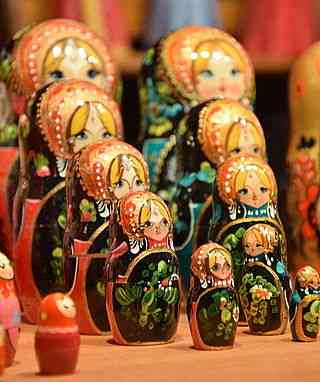
\includegraphics[width=1\textwidth,height=\textheight]{figures/poupeesrusses.jpg}
\end{column}
\end{columns}
\end{frame}

\begin{frame}[fragile]{Exemple}
\protect\hypertarget{exemple}{}
Comparons un modèle avec et sans \(X_6\).

Variable catégorielle à trois niveaux (deux coefficients associés à
\(\mathrm{I}(\mathrm{X}_{6}=2)\) et \(\mathrm{I}(\mathrm{X}_{6}=3)\).

\begin{Shaded}
\begin{Highlighting}[numbers=left,,]
\NormalTok{modele2 }\OtherTok{\textless{}{-}}  \FunctionTok{glm}\NormalTok{(y }\SpecialCharTok{\textasciitilde{}}\NormalTok{ x1 }\SpecialCharTok{+}\NormalTok{ x2 }\SpecialCharTok{+}\NormalTok{ x3 }\SpecialCharTok{+}\NormalTok{ x4 }\SpecialCharTok{+}\NormalTok{ x5 }\SpecialCharTok{+}\NormalTok{ x6,}
                 \AttributeTok{data =}\NormalTok{ hecmulti}\SpecialCharTok{::}\NormalTok{logit1,}
                 \AttributeTok{family =} \FunctionTok{binomial}\NormalTok{(}\AttributeTok{link =} \StringTok{"logit"}\NormalTok{))}
\NormalTok{modele3 }\OtherTok{\textless{}{-}}  \FunctionTok{glm}\NormalTok{(y }\SpecialCharTok{\textasciitilde{}}\NormalTok{ x1 }\SpecialCharTok{+}\NormalTok{ x2 }\SpecialCharTok{+}\NormalTok{ x3 }\SpecialCharTok{+}\NormalTok{ x4 }\SpecialCharTok{+}\NormalTok{ x5,}
                 \AttributeTok{data =}\NormalTok{ hecmulti}\SpecialCharTok{::}\NormalTok{logit1,}
                 \AttributeTok{family =} \FunctionTok{binomial}\NormalTok{(}\AttributeTok{link =} \StringTok{"logit"}\NormalTok{)) }
\end{Highlighting}
\end{Shaded}
\end{frame}

\begin{frame}{Test d'hypothèse}
\protect\hypertarget{test-dhypothuxe8se}{}
On teste l'hypothèse nulle
\(\mathscr{H}_0: \beta_{\mathrm{X}_6=2} = \beta_{\mathrm{X}_6=3} = 0\)
(soit \(k=2\) restrictions).

L'hypothèse alternative est qu'au moins un des coefficients est non-nul.

Si la valeur \(p\) est inférieure au seuil de signification, typiquement
\(\alpha = 0.05\), on rejette l'hypothèse nulle.

\begin{itemize}
\tightlist
\item
  on conclut que la variable explicative \(\mathrm{X}_6\) améliore
  significativement l'ajustement du modèle.
\end{itemize}
\end{frame}

\begin{frame}{Rapport de vraisemblance}
\protect\hypertarget{rapport-de-vraisemblance}{}
Le test est basé sur la statistique \begin{align*}
 D = -2\{\ell(\widehat{\boldsymbol{\beta}}_0)-\ell(\widehat{\boldsymbol{\beta}})\}.
\end{align*}

Cette différence \(D\), lorsque l'hypothèse \(\mathscr{H}_0\) est vraie,
suit approximativement une loi khi-deux \(\chi^2_k\).
\end{frame}

\begin{frame}[fragile]{Exemple de test}
\protect\hypertarget{exemple-de-test}{}
\footnotesize

\begin{Shaded}
\begin{Highlighting}[numbers=left,,]
\CommentTok{\# modèle 2 (alternative), modèle 3 (nulle)}
\FunctionTok{anova}\NormalTok{(modele3, modele2, }\AttributeTok{test =} \StringTok{"LR"}\NormalTok{)}
\end{Highlighting}
\end{Shaded}

\begin{verbatim}
Analysis of Deviance Table

Model 1: y ~ x1 + x2 + x3 + x4 + x5
Model 2: y ~ x1 + x2 + x3 + x4 + x5 + x6
  Resid. Df Resid. Dev Df Deviance  Pr(>Chi)    
1       488     566.45                          
2       486     516.20  2   50.251 1.225e-11 ***
---
Signif. codes:  0 '***' 0.001 '**' 0.01 '*' 0.05 '.' 0.1 ' ' 1
\end{verbatim}

\begin{Shaded}
\begin{Highlighting}[numbers=left,,]
\DocumentationTok{\#\# Deviance = {-}2*log vraisemblance}
\NormalTok{rvrais }\OtherTok{\textless{}{-}}\NormalTok{ modele3}\SpecialCharTok{$}\NormalTok{deviance }\SpecialCharTok{{-}}\NormalTok{ modele2}\SpecialCharTok{$}\NormalTok{deviance}
\FunctionTok{pchisq}\NormalTok{(rvrais, }\AttributeTok{df =} \DecValTok{2}\NormalTok{, }\AttributeTok{lower.tail =} \ConstantTok{FALSE}\NormalTok{) }\CommentTok{\# valeur{-}p}
\end{Highlighting}
\end{Shaded}

\begin{verbatim}
[1] 1.225046e-11
\end{verbatim}

\normalsize
\end{frame}

\begin{frame}[fragile]{Tester la significativité des variables}
\protect\hypertarget{tester-la-significativituxe9-des-variables}{}
Si un paramètre n'est pas significativement différent de 0, cela veut
dire qu'il n'y a pas de lien significatif entre la variable et la
réponse \emph{une fois que les autres variables} sont dans le modèle.

\footnotesize

\begin{Shaded}
\begin{Highlighting}[numbers=left,,]
\NormalTok{car}\SpecialCharTok{::}\FunctionTok{Anova}\NormalTok{(modele2, }\AttributeTok{type =} \StringTok{"3"}\NormalTok{)}
\end{Highlighting}
\end{Shaded}

\begin{verbatim}
Analysis of Deviance Table (Type III tests)

Response: y
   LR Chisq Df Pr(>Chisq)    
x1    4.291  4     0.3681    
x2   32.912  4  1.245e-06 ***
x3   29.878  1  4.601e-08 ***
x4   42.957  1  5.597e-11 ***
x5   36.731  1  1.356e-09 ***
x6   50.251  2  1.225e-11 ***
---
Signif. codes:  0 '***' 0.001 '**' 0.01 '*' 0.05 '.' 0.1 ' ' 1
\end{verbatim}

\normalsize
\end{frame}

\begin{frame}[fragile]{Intervalles de confiance pour coefficients}
\protect\hypertarget{intervalles-de-confiance-pour-coefficients}{}
On peut aussi considérer des intervalles de confiance pour les
coefficients individuels.

Ceux obtenus par défaut dans \textbf{R} sont appelés \emph{intervalles
de confiance de vraisemblance profilée}.

\begin{Shaded}
\begin{Highlighting}[numbers=left,,]
\FunctionTok{confint}\NormalTok{(modele2)      }\CommentTok{\# IC pour beta}
\FunctionTok{exp}\NormalTok{(}\FunctionTok{confint}\NormalTok{(modele2)) }\CommentTok{\# IC pour exp(beta)}
\end{Highlighting}
\end{Shaded}

Ces intervalles sont invariants aux reparamétrisation: si \([b_i, b_s]\)
est l'intervalle de vraisemblance profilée pour \(\beta\), l'intervalle
pour \(\exp(\beta)\) est simplement \([\exp(b_i), \exp(b_s)]\).
\end{frame}

\begin{frame}{Intervalles de confiance}
\protect\hypertarget{intervalles-de-confiance}{}
\begin{figure}

{\centering \includegraphics[width=0.8\textwidth,height=\textheight]{MATH60602-diapos5_files/figure-beamer/fig-confint-modele2-logist-1.pdf}

}

\caption{\label{fig-confint-modele2-logist}Intervalles de confiance
profilés de niveau 95\% pour les coefficients du modèle logistique
(échelle exponentielle).}

\end{figure}
\end{frame}

\begin{frame}{Tests et intervalles de confiances}
\protect\hypertarget{tests-et-intervalles-de-confiances}{}
Comme \(\exp(\cdot)\) est une transformation monotone croissante,
\[\beta>0 \quad \iff \quad \exp(\beta)>1.\]

Si la valeur postulée, par exemple \(\mathscr{H}_0: \beta_j=0\) ou
\(\exp(\beta_j)=1\), est dans l'intervalle de confiance de niveau
\(1-\alpha\), on ne rejette pas l'hypothèse nulle.
\end{frame}

\begin{frame}{Coefficients pour données complètes}
\protect\hypertarget{coefficients-pour-donnuxe9es-compluxe8tes}{}
\footnotesize

\hypertarget{tbl-logit1-complet}{}
\setlength{\LTpost}{0mm}
\begin{longtable}{lccc}
\caption{\label{tbl-logit1-complet}Modèle logistique avec toutes les variables catégorielles. }\tabularnewline

\toprule
variables & cote\textsuperscript{\textit{1}} & IC 95\%\textsuperscript{\textit{1}} & valeur-p \\ 
\midrule
x1 &  &  & 0.4 \\ 
    1 & — & — &  \\ 
    2 & 0.44 & 0.18, 1.06 &  \\ 
    3 & 0.51 & 0.21, 1.21 &  \\ 
    4 & 0.51 & 0.21, 1.25 &  \\ 
    5 & 0.70 & 0.27, 1.80 &  \\ 
x2 &  &  & <0.001 \\ 
    1 & — & — &  \\ 
    2 & 0.83 & 0.38, 1.82 &  \\ 
    3 & 0.57 & 0.25, 1.31 &  \\ 
    4 & 0.09 & 0.03, 0.25 &  \\ 
    5 & 0.26 & 0.08, 0.84 &  \\ 
x3 &  &  & <0.001 \\ 
    0 & — & — &  \\ 
    1 & 3.85 & 2.34, 6.50 &  \\ 
\bottomrule
\end{longtable}
\begin{minipage}{\linewidth}
\textsuperscript{\textit{1}}cote = rapport de cote, IC = intervalle de confiance\\
\end{minipage}

\normalsize
\end{frame}

\begin{frame}{Coefficients pour données complètes}
\protect\hypertarget{coefficients-pour-donnuxe9es-compluxe8tes-1}{}
\footnotesize

\hypertarget{tbl-logit1-complet2}{}
\setlength{\LTpost}{0mm}
\begin{longtable}{lccc}
\caption{\label{tbl-logit1-complet2}Modèle logistique avec toutes les variables catégorielles. }\tabularnewline

\toprule
variables & cote\textsuperscript{\textit{1}} & IC 95\%\textsuperscript{\textit{1}} & valeur-p \\ 
\midrule
x4 &  &  & <0.001 \\ 
    0 & — & — &  \\ 
    1 & 6.24 & 3.53, 11.4 &  \\ 
x5 & 1.12 & 1.08, 1.16 & <0.001 \\ 
x6 &  &  & <0.001 \\ 
    1 & — & — &  \\ 
    2 & 0.25 & 0.13, 0.49 &  \\ 
    3 & 0.09 & 0.04, 0.18 &  \\ 
\bottomrule
\end{longtable}
\begin{minipage}{\linewidth}
\textsuperscript{\textit{1}}cote = rapport de cote, IC = intervalle de confiance\\
\end{minipage}
\end{frame}

\begin{frame}{Multicolinéarité}
\protect\hypertarget{multicolinuxe9arituxe9}{}
Il est difficile de départager l'effet individuel d'une variable
explicative lorsqu'elle est fortement corrélée avec d'autres.

La multicollinéarité ne dépend pas de la variable réponse \(Y\), mais de
la matrice \(\mathbf{X}\) du modèle.
\end{frame}

\begin{frame}[fragile]{Multicolinéarité pour PRCA}
\protect\hypertarget{multicolinuxe9arituxe9-pour-prca}{}
Mêmes diagnostics qu'en régression linéaire: considérer les facteurs
d'inflation de la variance (\texttt{car::vif}).

\begin{Shaded}
\begin{Highlighting}[numbers=left,,]
\NormalTok{car}\SpecialCharTok{::}\FunctionTok{vif}\NormalTok{(modele2)}
\end{Highlighting}
\end{Shaded}

\begin{verbatim}
       GVIF Df GVIF^(1/(2*Df))
x1 1.698464  4        1.068457
x2 1.852841  4        1.080139
x3 1.450100  1        1.204201
x4 1.491202  1        1.221148
x5 1.219334  1        1.104234
x6 1.179133  2        1.042055
\end{verbatim}

Pas d'inquiétude ici, coefficients faibles (inférieurs à 5)
\end{frame}

\begin{frame}{Dichotomiser des variables continues}
\protect\hypertarget{dichotomiser-des-variables-continues}{}
Si \(Y\) est continue et qu'on cherche à estimer
\(\Pr(Y> c \mid \mathbf{X})\) pour une valeur \(c\) donnée, il n'est
\textbf{pas} recommandé de dichotomiser \(Y\) via

\begin{align*}
Y^{*} = \begin{cases}
1, & Y > c; \\
0, & Y \leq c.
\end{cases}
\end{align*}

et d'ajuster une régression logistique.

Pourquoi? \textbf{On perd de l'information}.
\end{frame}

\begin{frame}[fragile]{Probabilité de dépassement}
\protect\hypertarget{probabilituxe9-de-duxe9passement}{}
On peut estimer plutôt une régression linéaire et prendre
\[\Pr(Y > c \mid \mathbf{X}) = \Phi\left(\frac{\widehat{\mu}-c}{\widehat{\sigma}}\right),\]

où

\begin{itemize}
\tightlist
\item
  \(\widehat{\mu}=\widehat{\beta}_0 + \cdots + \beta_p\mathrm{X}_p\) est
  la moyenne prédite pour le profil donné,
\item
  \(\widehat{\sigma}\) est l'estimation de l'écart-type
\item
  \(\Phi(\cdot)\) est la fonction de répartition d'une loi normale
  standard (\texttt{pnorm} dans \textbf{R})
\end{itemize}
\end{frame}

\begin{frame}{Modèle linéaire et probabilité d'excès}
\protect\hypertarget{moduxe8le-linuxe9aire-et-probabilituxe9-dexcuxe8s}{}
\begin{figure}

{\centering \includegraphics[width=0.8\textwidth,height=\textheight]{MATH60602-diapos5_files/figure-beamer/fig-density-normalcurves-1.pdf}

}

\caption{\label{fig-density-normalcurves}Régression linéaire simple et
densité normale à différentes valeurs de \(x\).}

\end{figure}
\end{frame}

\begin{frame}{Récapitulatif}
\protect\hypertarget{ruxe9capitulatif}{}
\begin{itemize}
\tightlist
\item
  Une régression logistique sert à modéliser la moyenne de
  \textbf{variables catégorielles}, typiquement binaires.
\item
  C'est un cas particulier d'un modèle de régression linéaire
  généralisée (GLM)
\end{itemize}
\end{frame}

\begin{frame}{Récapitulatif}
\protect\hypertarget{ruxe9capitulatif-1}{}
Le modèle est interprétable à l'échelle de la cote

\begin{itemize}
\tightlist
\item
  La cote donne le rapport probabilité de réussite (1) sur probabilité
  d'échec (0)
\item
  Interprétation en terme de

  \begin{itemize}
  \tightlist
  \item
    pourcentage d'augmentation si \(\exp(\widehat{\beta}) > 1\), avec
    \(\exp(\widehat{\beta})-1\).
  \item
    pourcentage de diminution si \(\exp(\widehat{\beta}) < 1\), avec
    \(1-\exp(\widehat{\beta})\)
  \end{itemize}
\end{itemize}
\end{frame}

\begin{frame}{Récapitulatif}
\protect\hypertarget{ruxe9capitulatif-2}{}
\begin{itemize}
\tightlist
\item
  Estimation par maximum de vraisemblance
\item
  Tests d'hypothèse comparent modèles emboîtés

  \begin{itemize}
  \tightlist
  \item
    loi nulle asymptotique \(\chi^2\)
  \item
    degrés de liberté égal au nombre de restrictions
  \end{itemize}
\item
  Intervalles de confiance de vraisemblance profilée

  \begin{itemize}
  \tightlist
  \item
    invariants aux reparamétrisations
  \end{itemize}
\end{itemize}
\end{frame}



\end{document}
